\section{Introducción}

Esta guía introduce los fundamentos de la \emph{visión por computadora} basada en
aprendizaje profundo y los aplica a un problema de clasificación de imágenes con
\emph{redes neuronales convolucionales} (CNN). Constituye la \textbf{Parte~1} del
laboratorio: se entrena una CNN \emph{desde cero}; la Parte~2 introducirá el
aprendizaje por transferencia sobre el mismo dominio.

\textbf{Materiales.} Python 3.10 con el entorno del laboratorio; el dataset de
botellas provisto en \texttt{data/botellas/}; y los tres notebooks de la carpeta
\texttt{parte1\_ia/} (Notebook~1 a Notebook~3). Cada notebook explica su código en
detalle; esta guía es la referencia teórica y describe \emph{qué} se hace y
\emph{cuánto} aporta a la evaluación.

\section{Preparación del entorno en VS Code}

El único requisito delicado es usar un entorno virtual con la \textbf{versión correcta de
Python} (3.10 o 3.11): con otra versión, TensorFlow no se instala correctamente.

\begin{enumerate}
  \item Abrir la carpeta del proyecto en \textbf{Visual Studio Code}.
  \item \emph{Command Palette} (\texttt{Ctrl+Shift+P}) $\rightarrow$
        \texttt{Python: Create Environment} $\rightarrow$ \texttt{Venv} $\rightarrow$ elegir
        un intérprete \textbf{Python 3.10} o \textbf{3.11}. Cuando VS Code lo solicite,
        marcar \texttt{requirements.txt} para que instale las dependencias en ese entorno.
  \item En cada notebook, \texttt{Select Kernel} (arriba a la derecha) y elegir el entorno
        \texttt{.venv} recién creado.
\end{enumerate}

Con el entorno correcto seleccionado, las celdas de \texttt{import} de los notebooks
funcionan directamente (las dependencias ya quedaron instaladas al crear el entorno). Para
confirmar la versión:

\begin{lstlisting}[language=Python]
import sys, tensorflow as tf
print(sys.version)        # 3.10.x o 3.11.x
print(tf.__version__)     # 2.20.0
\end{lstlisting}

\section{Redes neuronales convolucionales}

Una CNN aprende a extraer características visuales directamente de los píxeles, sin
ingeniería manual de \emph{features}. Se compone de tres tipos de capas
(Figura~\ref{fig:cnn}):

\begin{itemize}
  \item \textbf{Convolución} (\texttt{Conv2D}): aplica filtros que se deslizan sobre la
        imagen y detectan patrones locales ---bordes, texturas, formas---. Los filtros
        se aprenden durante el entrenamiento (Figura~\ref{fig:conv}).
  \item \textbf{Pooling} (\texttt{MaxPooling2D}): reduce la resolución conservando la
        información dominante, lo que aporta robustez y disminuye el cómputo
        (Figura~\ref{fig:pool}).
  \item \textbf{Capas densas} (\texttt{Dense}): combinan las características extraídas; la
        capa de salida usa \emph{softmax} para producir una probabilidad por clase.
\end{itemize}

La función de activación \emph{ReLU} introduce la no linealidad entre capas; sin ella la
red colapsaría a una única transformación lineal (Figura~\ref{fig:act}).

\begin{figure}[h]
\centering
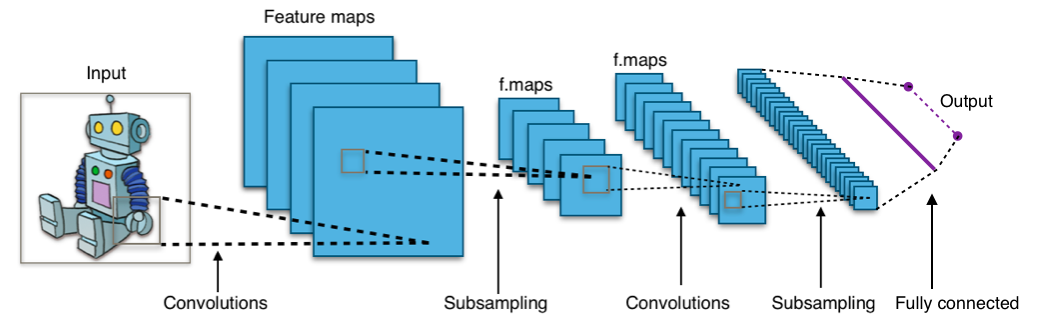
\includegraphics[width=0.92\textwidth]{../docs/assets/g1/typical_cnn_wikimedia.png}
\caption{Arquitectura típica de una CNN: bloques de convolución y pooling extraen características de complejidad creciente; las capas densas producen la clasificación. Fuente: Wikimedia Commons (CC BY-SA).}
\label{fig:cnn}
\end{figure}

\begin{figure}[h]
\centering
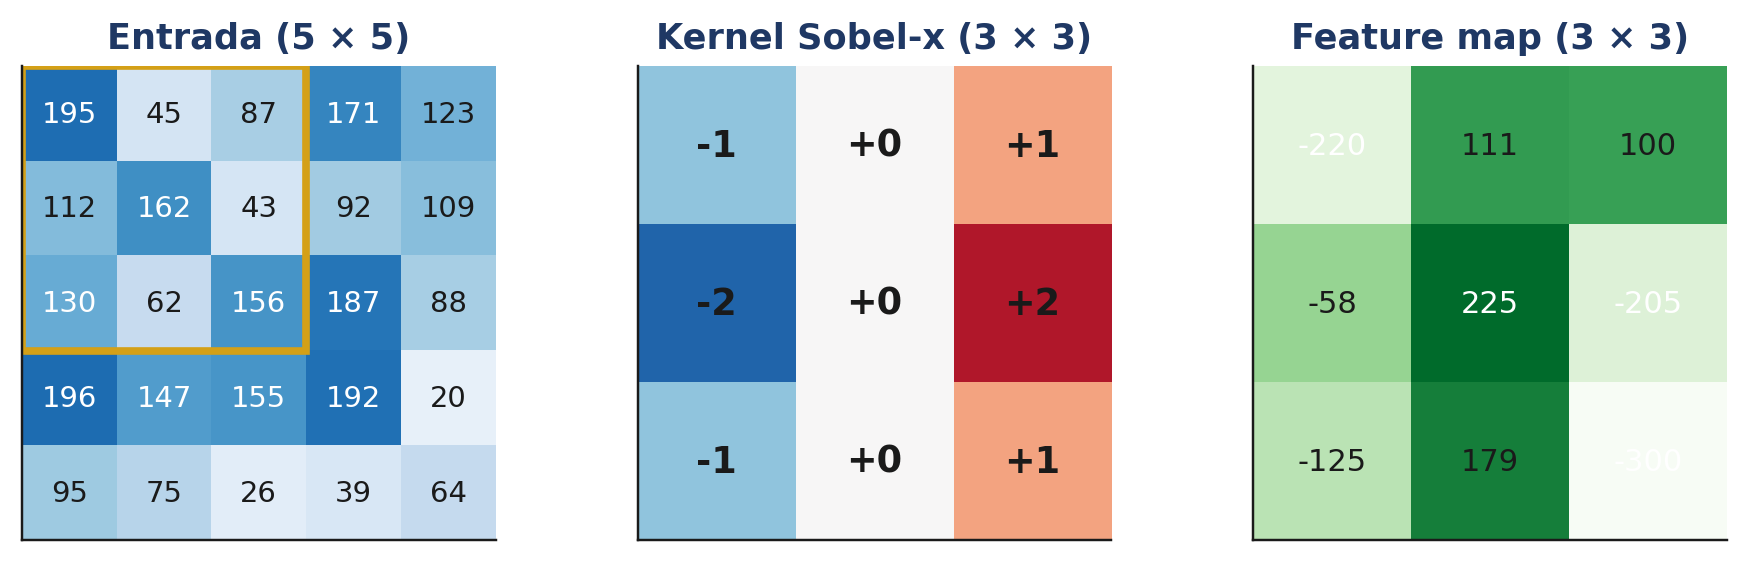
\includegraphics[width=0.8\textwidth]{../docs/assets/g1/g1_fig05_convolution.png}
\caption{Operación de convolución: un filtro recorre la imagen y produce un mapa de características. Fuente: Stanford CS231n.}
\label{fig:conv}
\end{figure}

\begin{figure}[h]
\centering
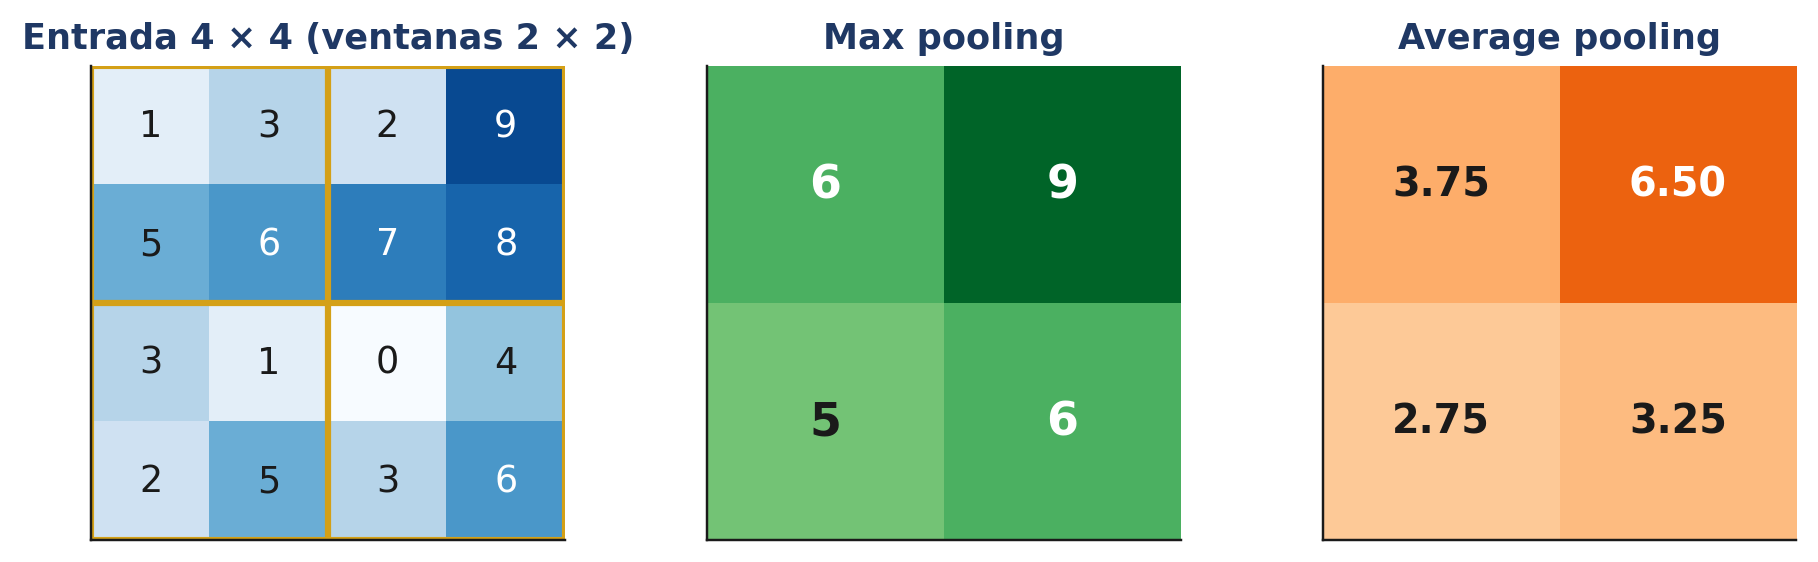
\includegraphics[width=0.78\textwidth]{../docs/assets/g1/g1_fig07_pooling.png}
\caption{Max pooling: cada región se resume por su valor máximo, reduciendo la resolución. Fuente: elaboración propia.}
\label{fig:pool}
\end{figure}

\begin{figure}[h]
\centering
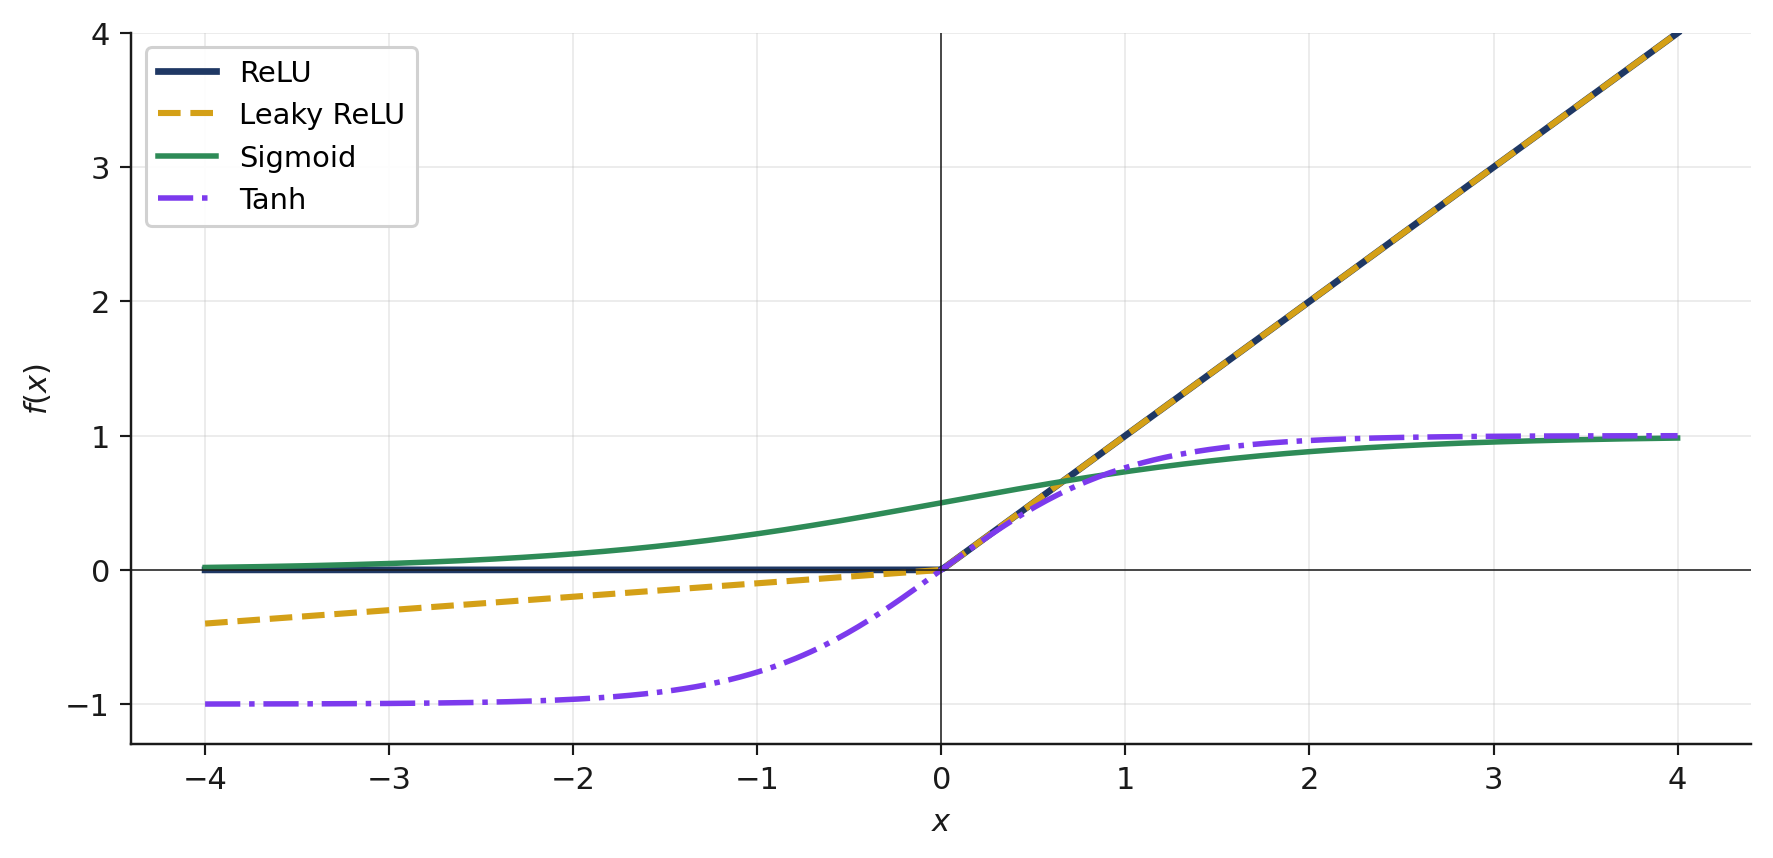
\includegraphics[width=0.78\textwidth]{../docs/assets/g1/g1_fig08_activations.png}
\caption{Funciones de activación habituales. \emph{ReLU} es la más usada en capas convolucionales. Fuente: elaboración propia.}
\label{fig:act}
\end{figure}

\section{Entrenamiento y evaluación}

El entrenamiento ajusta los filtros minimizando una \emph{función de pérdida}
(\emph{categorical crossentropy} para clasificación multiclase) mediante
\emph{backpropagation} y un optimizador (\emph{Adam} por defecto). El proceso se repite
durante varias \emph{épocas} sobre lotes (\emph{batches}) de imágenes.

El desempeño se mide sobre un conjunto de \textbf{validación} independiente. La
\emph{accuracy} y la \textbf{matriz de confusión} revelan no solo cuánto acierta el
modelo, sino dónde se confunde. Si la accuracy en entrenamiento es alta pero la de
validación es baja, el modelo sufre \emph{overfitting}: memoriza en lugar de generalizar.

\section{Aumentación de datos}

La \emph{data augmentation} genera variaciones de las imágenes de entrenamiento
---rotaciones, desplazamientos, cambios de brillo, zoom--- para que el modelo generalice
mejor con pocos datos. Es la primera defensa contra el \emph{overfitting} sin modificar
la arquitectura.

% =============================================================================
\section{Experiencia guiada}\label{sec:guiada}

El trabajo se desarrolla en tres notebooks que la pareja ejecuta y completa. La
indicación es la misma para todos: \textbf{ejecutar el notebook de principio a fin,
completar las celdas marcadas como \emph{«completar»} y responder por escrito las
preguntas conceptuales}. Como los notebooks ya vienen implementados, \textbf{la nota
evalúa la comprensión}: las respuestas a las preguntas conceptuales y la interpretación y
justificación de los resultados, no la simple ejecución. La rúbrica completa está en la
\emph{Ficha de Evaluación}: la Parte~1 aporta \textbf{10 puntos} y la Parte~2 otros 10,
para una nota sobre 20.

Los Notebooks 1 y 2 usan el dataset de botellas (vidrio/plástico) provisto; el Notebook~3
usa un dataset de tapitas construido por la propia pareja. El dataset se organiza en
subcarpetas por clase dentro de \texttt{train/} y \texttt{validation/}, de modo que
\texttt{ImageDataGenerator} infiera las etiquetas automáticamente:

\begin{center}
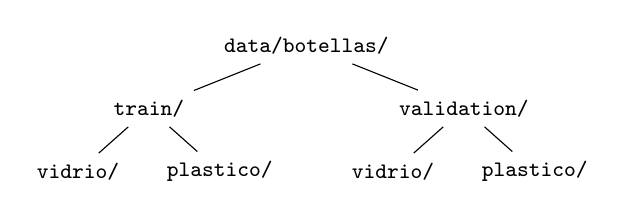
\begin{tikzpicture}[
  every node/.style={font=\footnotesize\ttfamily},
  level distance=8mm, sibling distance=20mm,
  level 1/.style={sibling distance=40mm}, level 2/.style={sibling distance=18mm},
]
\node {data/botellas/}
  child { node {train/} child { node {vidrio/} } child { node {plastico/} } }
  child { node {validation/} child { node {vidrio/} } child { node {plastico/} } };
\end{tikzpicture}
\end{center}

\subsection{Notebook 1: CNN desde cero}

Recorre el ciclo completo de una CNN entrenada desde cero: carga del dataset, definición
y compilación de la arquitectura (Figura~\ref{fig:arch}: bloques
\texttt{Conv2D}\,+\,\texttt{MaxPooling2D}, \texttt{Flatten}, capa densa con \emph{dropout}
y salida \emph{softmax}), entrenamiento, evaluación con matriz de confusión y predicción
sobre imágenes propias (Figuras~\ref{fig:curvas} y~\ref{fig:confmat}).

\begin{figure}[h]
\centering
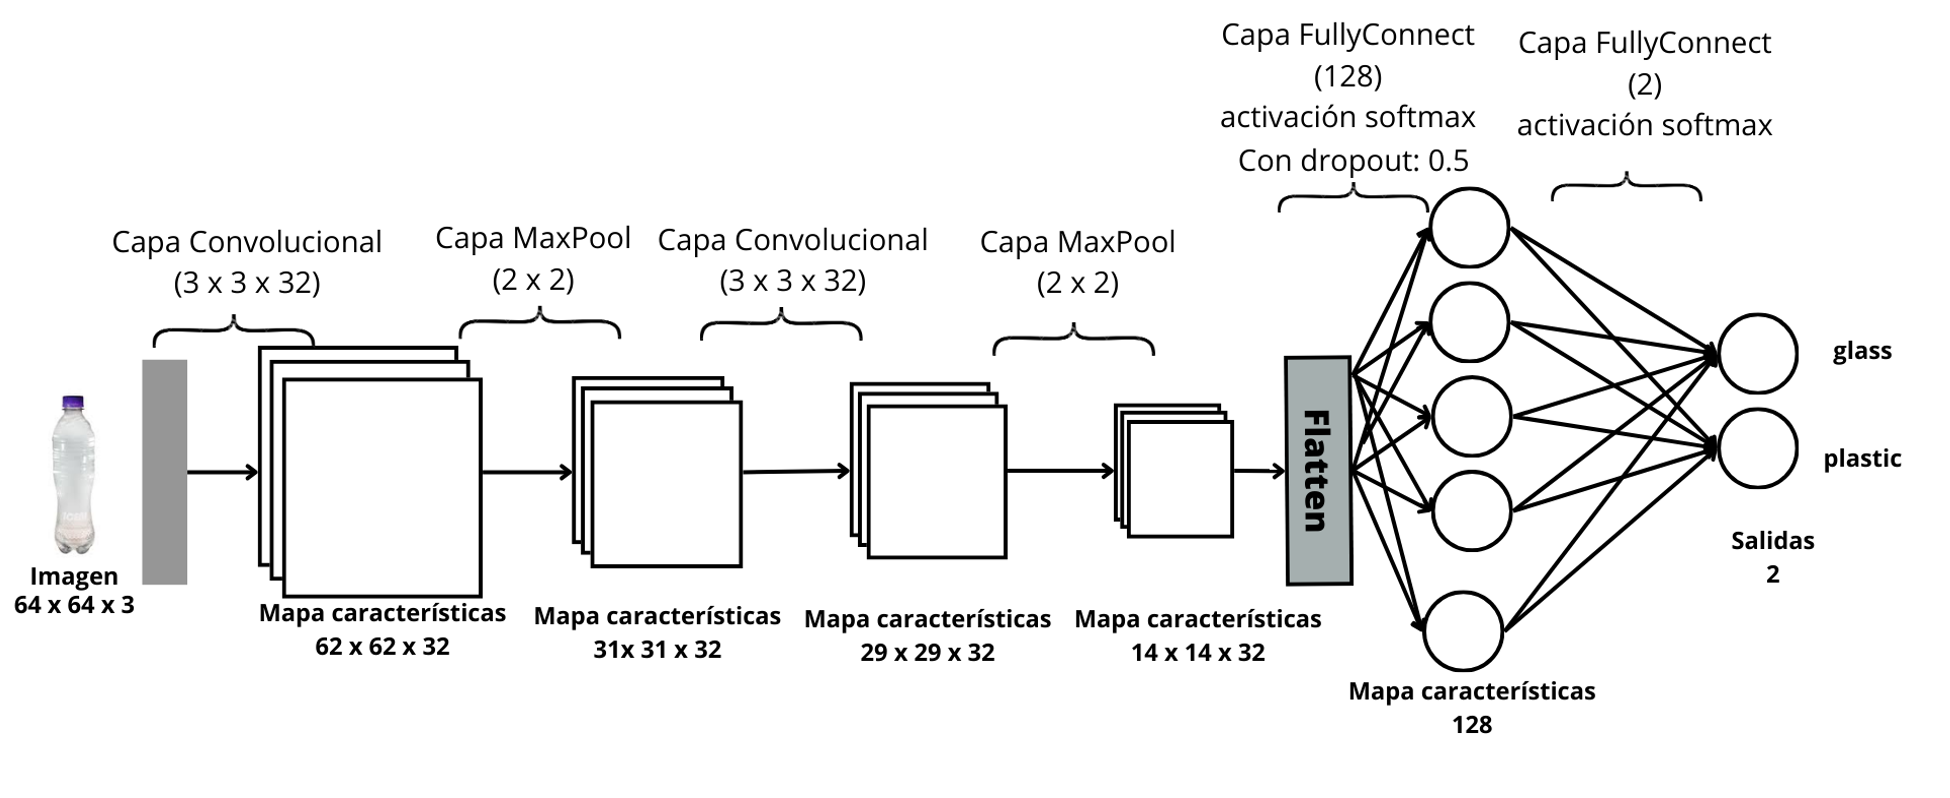
\includegraphics[width=0.95\textwidth]{../docs/assets/g1/arquitectura_botellas.png}
\caption{Arquitectura de la CNN del laboratorio. Fuente: elaboración propia (NN-SVG).}
\label{fig:arch}
\end{figure}

\renewcommand{\arraystretch}{1.3}
\begin{tabularx}{\textwidth}{@{}p{6.2cm} X r@{}}
\toprule
\textbf{Etapa (secciones del notebook)} & \textbf{Qué se realiza} & \textbf{Puntos} \\
\midrule
1. Arquitectura y entrenamiento \newline (secciones 3--6)
  & Definir y compilar la CNN, entrenar y analizar las curvas de \emph{loss}/\emph{accuracy} y la matriz de confusión sobre validación.
  & 1.5 \\
2. Evaluación con datos propios \newline (sección 7)
  & Clasificar cuatro fotografías capturadas por la pareja en condiciones variadas e identificar aciertos y fallos.
  & 1.5 \\
\bottomrule
\end{tabularx}
\renewcommand{\arraystretch}{1}

\begin{figure}[h]
\centering
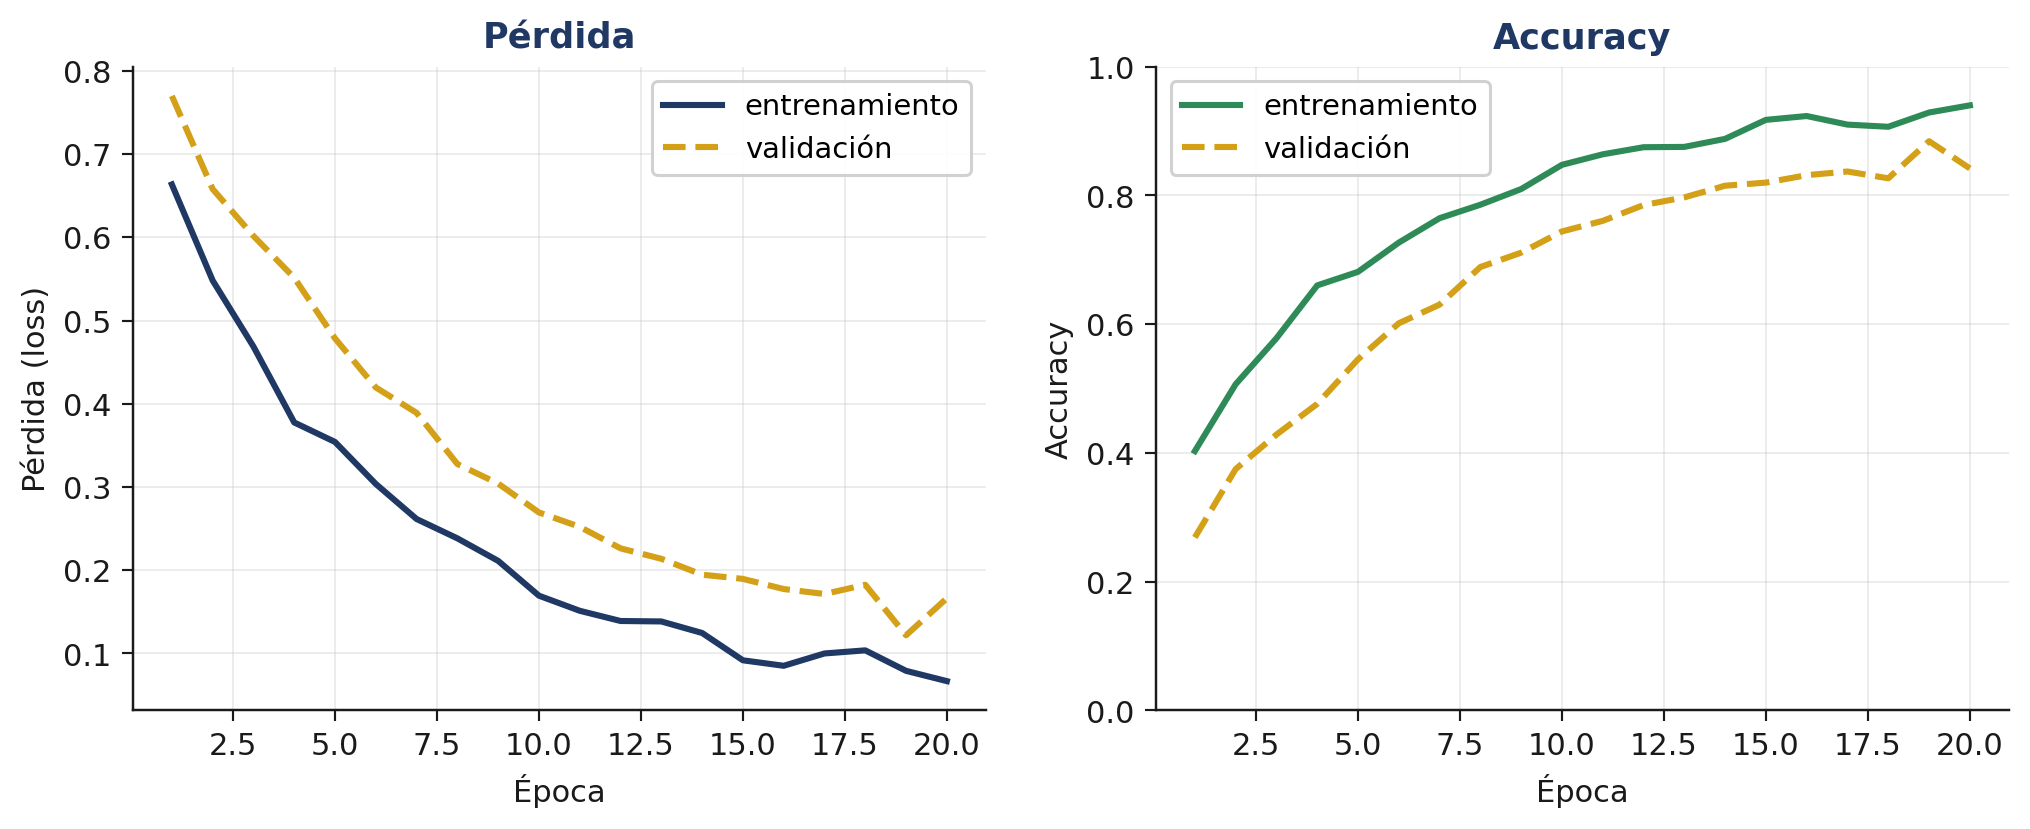
\includegraphics[width=0.82\textwidth]{../docs/assets/g1/g1_fig12_training_curves.png}
\caption{Curvas de aprendizaje esperadas sobre el dataset de botellas. Fuente: elaboración propia.}
\label{fig:curvas}
\end{figure}

\begin{figure}[h]
\centering
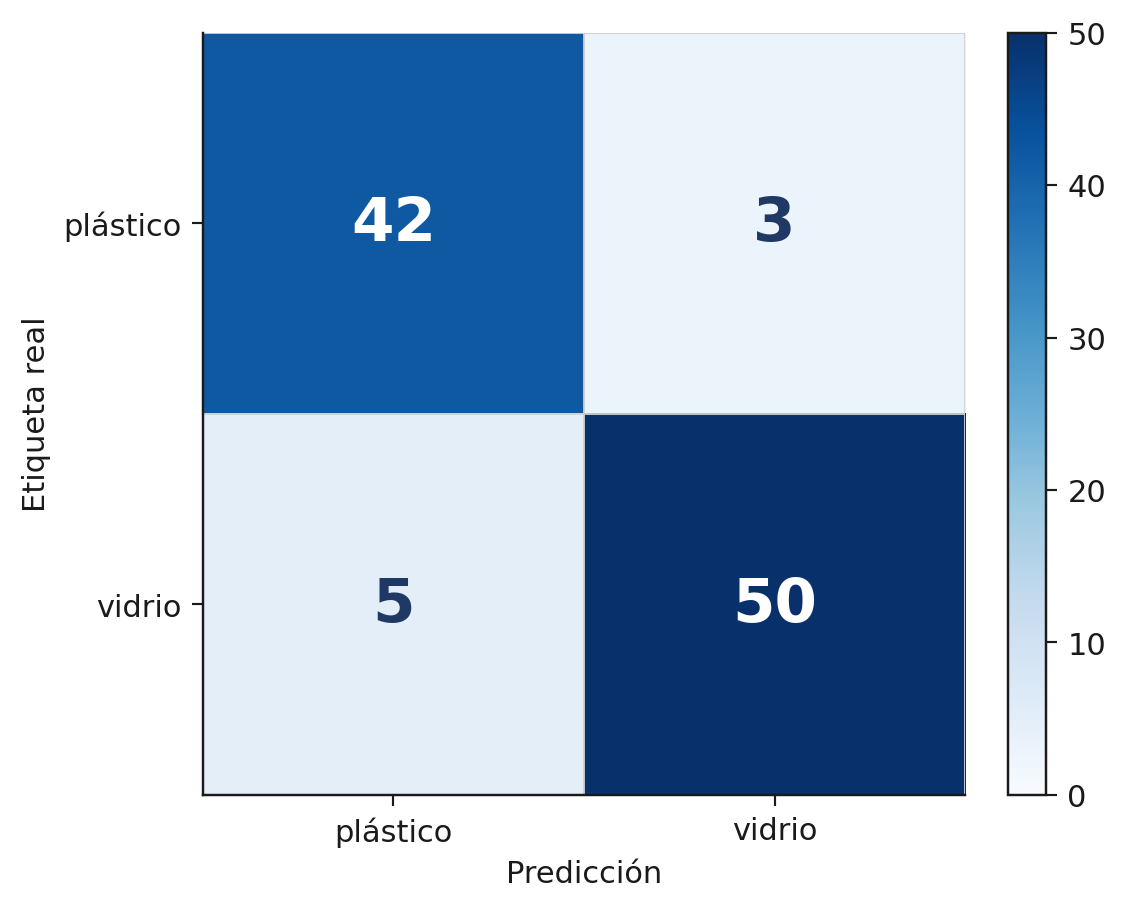
\includegraphics[width=0.45\textwidth]{../docs/assets/g1/g1_fig11_confmat.png}
\caption{Matriz de confusión sobre validación: la diagonal son aciertos. Fuente: elaboración propia.}
\label{fig:confmat}
\end{figure}

\subsection{Notebook 2: aumentación de datos}

Retoma el clasificador anterior para evidenciar y mitigar el \emph{overfitting}: reproduce
el sobreajuste del modelo base, selecciona transformaciones de aumentación pertinentes,
reentrena y compara el desempeño frente al modelo sin aumentar.

\renewcommand{\arraystretch}{1.3}
\begin{tabularx}{\textwidth}{@{}p{6.2cm} X r@{}}
\toprule
\textbf{Etapa (secciones del notebook)} & \textbf{Qué se realiza} & \textbf{Puntos} \\
\midrule
3. Data augmentation \newline (secciones 2--5)
  & Diagnosticar el \emph{overfitting} del modelo base, seleccionar transformaciones justificadas, reentrenar y comparar curvas frente al modelo base.
  & 2.5 \\
\bottomrule
\end{tabularx}
\renewcommand{\arraystretch}{1}

\subsection{Notebook 3: clasificador de tapitas}

Introduce un dataset propio: tapitas de colores (\textbf{rojo}, \textbf{azul},
\textbf{amarillo}) más una clase \texttt{fondo} (imágenes sin tapita). La pareja graba un
video corto por color, el notebook extrae los \emph{frames} a \texttt{data/tapitas/<clase>/}
(descartando los borrosos), divide en \emph{train}/\emph{validation} y entrena una CNN desde
cero. El modelo se exporta a \texttt{modelos/} para reutilizarlo en la Parte~2.

\textbf{Protocolo de captura:} iluminación y fondos variados, distancia 10--40\,cm,
ángulos diversos, una sola tapita por imagen y al menos 50 muestras por clase.

\renewcommand{\arraystretch}{1.3}
\begin{tabularx}{\textwidth}{@{}p{6.2cm} X r@{}}
\toprule
\textbf{Etapa (pasos del notebook)} & \textbf{Qué se realiza} & \textbf{Puntos} \\
\midrule
4. Captura y preparación del dataset \newline (pasos 1--2)
  & Grabar un video por color, extraer los frames a \texttt{data/tapitas/} y reportar el conteo por clase.
  & 1.0 \\
5. Entrenamiento y evaluación CNN \newline (pasos 3--4)
  & Dividir \emph{train}/\emph{validation}, entrenar la CNN, analizar curvas y matriz de confusión, y exportar el modelo.
  & 2.0 \\
\bottomrule
\end{tabularx}
\renewcommand{\arraystretch}{1}

\subsection{Cierre: discusión crítica}

A partir de los resultados, la pareja formula al menos dos hipótesis técnicas sobre las
causas de los errores (sesgos del dataset, sensibilidad a la iluminación, límites de la
arquitectura) y propone dos estrategias de mejora sin cambiar la arquitectura. Se
documenta en la Ficha de Evaluación (\textbf{1.5 puntos}).

\begin{center}
\renewcommand{\arraystretch}{1.3}
\begin{tabular}{@{}lr@{}}
\toprule
\textbf{Distribución de la nota de la Parte 1} & \textbf{Puntos} \\
\midrule
Notebook 1 --- \texttt{notebook1\_cnn\_desde\_cero.ipynb}      & 3.0 \\
Notebook 2 --- \texttt{notebook2\_data\_augmentation.ipynb}    & 2.5 \\
Notebook 3 --- \texttt{notebook3\_clasificador\_tapitas.ipynb} & 3.0 \\
Discusión crítica                                              & 1.5 \\
\midrule
\textbf{Total Parte 1} & \textbf{10.0} \\
\bottomrule
\end{tabular}
\renewcommand{\arraystretch}{1}
\end{center}

% =============================================================================
\section{Cierre: el límite del entrenamiento desde cero}\label{sec:cierre}

La evaluación sobre datos propios suele revelar un resultado aleccionador: el modelo
alcanza buena \emph{accuracy} en validación, pero \textbf{falla ante condiciones reales}
de iluminación, fondo o ángulo distintas a las del entrenamiento. La aumentación
(Notebook~2) mitiga el problema pero no lo resuelve: una CNN entrenada desde cero necesita
muchas más imágenes de las que es razonable capturar a mano.

Ese es el límite que motiva la \textbf{Parte 2}: en lugar de aprender todos los filtros
desde cero, se parte de una red ya entrenada sobre millones de imágenes y se reutiliza su
conocimiento ---\emph{aprendizaje por transferencia}---, obteniendo clasificadores robustos
con apenas unos cientos de imágenes por clase. Sobre esa técnica se construye el sistema de
control de calidad de la segunda parte, reutilizando el dataset de tapitas del Notebook~3.
